\section{Algorithmic options for fitting arbitrary posterior approximations}
\label{sec:chap5_wild_solutions}
The implicit distributions discussed in Section \ref{sec:chap5_wild_dist} cannot be fitted using many existing approximate inference methods such as MC-VI. In this section, we discuss four algorithmic options for training these approximations to the posterior.\footnote{Again we note here that the discussed options are applicable to tractable $q$ distributions as well. See discussions in the remark in Section \ref{sec:chap5_wild_concept}.}
%
One of the schemes is further developed in the next chapter. Other approaches that my colleagues and I proposed (following these ideas) include \citet{li:dropout2017, li:amcmc2017} which are not presented in the thesis due to page limit. 

\subsection{Energy approximation}
Assume $q$ is reparameterisable,\footnote{For non-reparameterisable distributions $\nabla_{\bm{\phi}} \f$ can be computed with further approximations such as the generalised reparameterisation trick \citep{ruiz:generalized_reparam2016}.} i.e. $\z \sim q_{\vparam}(\z|\x) \Leftrightarrow \z = \f_{\vparam}(\x)$.
%
Then by the chain rule, the gradient of a given objective function $\mathcal{L}(\vparam)$ w.r.t.~$\vparam$ is $\nabla_{\bm{\phi}} \mathcal{L} = \nabla_{\bm{\phi}} \f \nabla_{\f} \mathcal{L} $. Therefore, if we have an approximation $\hat{\mathcal{L}}$ to the objective function, then we can approximate the gradient as $\nabla_{\bm{\phi}} \mathcal{L} \approx \nabla_{\bm{\phi}} \f \nabla_{\f} \hat{\mathcal{L}}$. We name this approach as \emph{energy/objective approximation}.

Since the loss function $\mathcal{L}(\vparam)$ is often defined as $\mathcal{L}(q_{\vparam})$, a naive method of energy approximation considers density estimation of $q_{\vparam}$ and a direct plug-in of the approximate density to the energy function. Typically a density estimator $\hat{q}$, e.g. kernel density estimators (KDE) \citep{fukunaga:mean_shift1975} or neural density estimators \citep{mackay:density1999, larochelle:nade2011}, is fitted to the samples $\{\bm{z}^k = \f(\bm{\epsilon}^k, \bm{x}) \} \sim q$, and the gradient of $\log q$ is approximated as $\nabla_{\bm{\phi}} \log q(\bm{z}|\bm{x}) \approx \nabla_{\bm{z}} \log \hat{q}(\bm{z}|\bm{x}) \nabla_{\bm{\phi}} \f$. One might even want to directly estimate $\log q$ if it turns out to be more accurate. However, practitioners should be careful with implementations using automatic differentiation tools, since the parameters of the density estimator $\hat{q}$ should not be differentiated through (even though they might depend on the samples $\bm{z}^k$). 

The next idea considers analytical approximations to (part of) the energy function, e.g.~the entropy term $\mathbb{H}[q]$ or the KL-divergence $\mathrm{KL}[q||p_0]$ in $\mathcal{L}_{\text{VI}}$, and let the MC approach handle the rest. In MC-dropout \citep{gal:dropout2016} $\mathrm{KL}[q||p_0]$ is approximated by an $\ell_2$ regulariser of the neural network weights. In \citet{li:dropout2017} we extended this framework to $\alpha$-divergence methods with further approximations. Due to the page limit, we skip the detailed discussions of this work.


A new direction for energy approximation applies density ratio estimation methods \citep{qin:ratio1998, sugiyama:ratio2009, sugiyama:ratio2012}. This is done by introducing an auxiliary distribution $\tilde{q}$ and rewriting the variational lower-bound:
\begin{equation}
 \quad \mathcal{L}_{\text{VI}}(\bm{\theta}, q; \bm{x}) =  \mathbb{E}_{q} \left[ \log \frac{p_0(\bm{z}) p(\bm{x}|\bm{z} ; \bm{\theta})}{\tilde{q}(\bm{z}|\bm{x})} + \log \frac{\tilde{q}(\bm{z}|\bm{x})}{q(\bm{z}|\bm{x})} \right].
\end{equation}
The auxiliary distribution $\tilde{q}$ is required to have tractable density and is easy to sample from. Then one can use sample-based density ratio estimation methods to fit an estimator $\tilde{R}$ to the ratio between $\tilde{q}$ and $q$. The gradient approximation for general $\tilde{q}$ distributions can be derived similarly as
\begin{equation}
 \nabla_{\bm{\phi}} \mathcal{L}_{\text{VI}} = \mathbb{E}_{q} \left[ \nabla_{\bm{\phi}} \log \frac{p_0(\bm{z}) p(\bm{x}|\bm{z}; \bm{\theta})}{\tilde{q}(\bm{z}|\bm{x})} + \nabla_{\bm{z}} \tilde{R}(\bm{z}) \nabla_{\bm{\phi}} \f \right].
\end{equation}
%
A simple example considers $\tilde{q} = p_0$ and the classification approach for ratio estimation. In short, we train a classifier 
$$D(\bm{z} \text{ sampled from } p_0 ~|~\z, \x) = (1 + \exp[-\tilde{R}(\bm{z})])^{-1}$$
to distinguish samples from $p_0$ and $q$. A related approach is the adversarial auto-encoder \citep{makhzani:adversarial_ae2015} which uses the prior distribution as an auxiliary. However, the objective function proposed in \citet{makhzani:adversarial_ae2015} replaces the $\mathrm{KL}[q||p_0]$ in the variational lower-bound with Jensen-Shannon divergence \citep{lin:jensen_shannon1991}, which lacks a justification from a Bayesian point of view.\footnote{An optimal transport \citep{villani:optimal_transport2008} perspective of adversarial auto-encoders is presented in \citet{tolstikhin:wae2018}. } Also the density ratio estimation idea can be extended to a sequence of auxiliary distributions (in a similar spirit to annealed importance sampling \citep{neal:ais2001}), which can also be adapted slowly during training to obtain a better approximation.

\vspace{1em}
\begin{tcolorbox}
\textbf{Remark} (concurrent work on the density ratio estimation idea)\textbf{.}
Since the presentation of the original material at the NIPS 2016 approximate inference workshop, this density ratio estimation proposal has also been independently considered in \cite{karaletsos:adversarial_mp2016, mescheder:avb2017, huszar:implicit2017, tran:implicit2017}. Specifically in the adversarial variational Bayes (AVB) paper \citep{mescheder:avb2017}, the authors first considered prior distribution as the auxiliary $\tilde{q}$, then discussed an advanced technique termed as \emph{adaptive contrast}, which takes $\tilde{q}$ as a Gaussian approximation to $q$. In this case the estimation of $\tilde{q}$ requires many samples from $q$ which can significantly slow down training. To address this issue, the authors further constructed a specific type of implicit $q$ distributions, which allows sharing of randomness between different $q(\z_n | \x_n)$ distributions and thus reducing the total number of MC samples computed on a mini-batch of data. This trick improves the approximation accuracy by a significant margin as density ratio estimation is accurate when the two distributions are similar to each other.
\end{tcolorbox}

\subsection{Direct gradient approximation}
\label{sec:chap5_grad_approx}
The recent development of machine learning algorithms, including VI and SG-MCMC, relies on advanced optimisation tools such as stochastic gradient descent with adaptive learning rates. Informally the optimisation procedure works as the following: given the current mini-batch of data, we first compute the gradients, then feed them to the optimiser to construct the final update of the training parameters. In the above energy approximation example, this gradient computation is done by first approximating the original objective function $\hat{\mathcal{L}} \approx \mathcal{L}$, then differentiating this approximate energy to obtain an approximate descending direction. However, even when $\hat{\mathcal{L}}$ approximates $\mathcal{L}$ very well at the points visited by gradient descent, the approximate gradient $\nabla_{\vparam} \hat{\mathcal{L}}$ can still be a poor estimator for the exact gradient $\nabla_{\vparam} \mathcal{L}$. We depict this phenomenon in Figure \ref{fig:chap_wild_loss_pathology}. Recall that practically, an optimiser only visits \emph{finite} number of locations in the parameter space. As one would typically use a deep neural network to approximate the exact loss function, without careful control the deep net can potentially overfit to the observed evaluations, leading to strongly biased gradient updates and bad local optima.

\begin{figure}
\centering
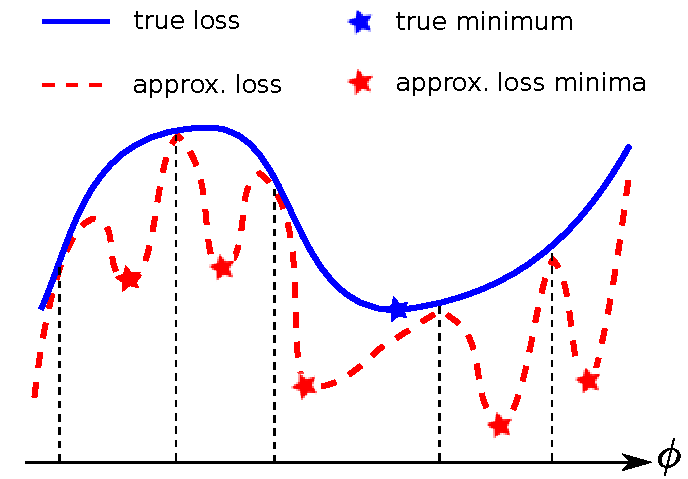
\includegraphics[width=0.5\linewidth]{Chapter5/approx_loss.pdf}
\caption{A visualisation of the exact/approximate loss. See main text for further intuition.}
\label{fig:chap_wild_loss_pathology}
\end{figure}

Here are two concrete examples for further explanation.

\begin{itemize}
\item Variational EM as an approximation to MLE. \\
The VAE algorithm can be viewed as an approximate MLE procedure, with the maximum likelihood objective $\mathcal{L}(\mparam) = \mathbb{E}_{\data}[\log p_{\mparam}(\x)]$ approximated by the variational lower-bound $\hat{\mathcal{L}}(\mparam, \vparam) = \mathbb{E}_{\data}[\mathcal{L}_{\text{VI}}(q_{\vparam}(\z | \x); \x)]$. As shown in the mean-field example in Section \ref{sec:chap4_mean_field}, this would bias the generative model $p_{\mparam}(\z | \x)$ towards simple solutions, unless $q_{\vparam}(\z | \x)$ perfectly approximates the exact posterior which is rarely the case. This issue is related to the ``hidden unit over-pruning'' problem \citep{burda:iwae2016, sonderby:ladder_vae2016}: even when $\z$ is of relatively high dimensions like a hundred, the VAE algorithm would turn off many of them, and learn a model which effectively uses much fewer units.

\item GAN training. \\
Recently generative adversarial networks (GANs) \citep{goodfellow:gan2014} have attracted large attention from the deep learning community. In a nutshell, the original GAN algorithm proposes training the generator $p_{\mparam}(\x)$ by minimising the Jensen-Shannon divergence
\begin{equation}
\min_{\mparam} \mathcal{L}(\mparam) = \mathrm{JS}[p_{\data} || p_{\mparam}] = \frac{1}{2} \mathrm{KL}\left[ p_{\data} || \frac{p_{\data} + p_{\mparam}}{2} \right] + \frac{1}{2} \mathrm{KL}\left[ p_{\mparam} || \frac{p_{\data} + p_{\mparam}}{2} \right].
\end{equation}
However, the generative model $p_{\mparam}(\x)$ is implicitly defined in an analogous way as the deterministic transform discussed above. Thus point-wise evaluation of $p_{\mparam}(\x)$ is intractable. Then the seminal GAN paper proposes approximating the Jenson-Shannon divergence \citep{lin:jensen_shannon1991} with a variational lower-bound, described by a \emph{discriminator}:
\begin{equation}
\min_{\mparam} \max_{\vparam} \hat{\mathcal{L}}(\mparam, \vparam) = \mathbb{E}_{\data} [\log D_{\vparam}(\x)] + \mathbb{E}_{p_{\mparam}} [\log (1 - D_{\vparam}(\x))].
\label{eq:chap5_original_gan}
\end{equation}
\cite{arjovsky:gan_problems2017} pointed out a fundamental problem with this approach: since both $p_{\data}$ and $p_{\mparam}$ have low-dimensional support in a high-dimensional space, the discriminator, if powerful enough (which is typically the case when using neural networks), is very likely to overfit, thus it can perfectly separate the two support sub-spaces and provide meaningless gradients. Then in their follow-up work \cite{arjovsky:wgan2017} proposed the Wasserstein GAN (WGAN), which uses Wasserstein distance \citep{villani:optimal_transport2008} as the training objective, and in this case, the approximate loss function turns out to be
\begin{equation}
\min_{\mparam} \max_{\vparam: || D_{\vparam}||_L \leq 1} \hat{\mathcal{L}}(\mparam, \vparam) = \mathbb{E}_{\data} [D_{\vparam}(\x)] - \mathbb{E}_{p_{\mparam}} [D_{\vparam}(\x)].
\label{eq:chap5_wgan}
\end{equation}
This modification, when adding more tricks to enforce the constraint $|| D_{\vparam}||_L \leq 1$ such as a gradient penalty \citep{gulrajani:wgan_gp2017}, has largely solved the instability issue of GAN training.

Another interesting explanation for why WGAN works is that the power of the discriminator, or the test function $D_{\vparam}$, has been restrained. On the other hand, in the original GAN case, over-fitting frequently happens, particularly at the beginning of training, as neural network classifiers can easily fit almost any data, even that with random labels as claimed by \cite{zhang:understanding2017}. Since smoothness is typically lost when over-fitting appears, it leads to poor approximations to the actual gradient and then a bad-performing model. Indeed \cite{kodali:dragan2017} also showed that the original GAN training can be stabilised when the discriminator is also constrained to be $1$-Lipschitz. 

\end{itemize}

From the above two examples, we see that the energy approximation approach can be problematic if not done in a correct way, therefore a \emph{direct gradient approximation} to the exact gradient might be preferred. There exists a rich literature on (non-parametric) derivative estimation \citep{stone:spline1985, zhou:spline2000, ruppert:lpr1994, fan:local_poly1996, debrabanter:lpr2013}; however, many of them require at least a noisy version of $\log q$ at the sampled locations, which is intractable in our case. Instead, \cite{singh:kernel_gradient1977} applied a kernel estimator directly to the first and higher order derivatives, and \cite{sasaki:gradient2015} improved upon this idea by performing kernel ridge regression directly on the derivatives. 
%
Also \cite{hyvarinen:score2005} considered score matching methods for approximating $\nabla_{\z} \log q(\z | \x)$, where follow-up papers \citep{sasaki:gradient2014, strathmann:kmc2015} derived kernel-based solutions and applied them to tasks such as approximate Bayesian computation (ABC) \citep{beaumont:abc2002}.
%
The core idea of these methods is the use of integration by parts to avoid evaluations of the actual gradients, making them applicable in our context. In Chapter \ref{chap:grad_approx} we will further discuss gradient approximation techniques and propose new gradient estimators for implicit models and wild approximate inference.

\vspace{1em}
\begin{tcolorbox}
\textbf{Remark} (denoising auto-encoder as a score function estimator)\textbf{.}
It has been shown in \citet{sarela:denoising2005, alain:denoising2014} that denoising auto-encoders (DAEs) \citep{vincent:denoising2008}, once trained, can be used to compute the score function approximately. Briefly speaking, a DAE learns to reconstruct a datum $\x$ from a corrupted input $\tilde{\x} = \x + \sigma \bm{\epsilon}, \bm{\epsilon} \sim \mathcal{N}(\bm{0}, \mathbf{I})$ by minimising the mean square error. Then the optimal DAE can be used to approximate the score function as $\nabla_{\x} \log p(\x) \approx \frac{1}{\sigma^2} (\text{DAE}^*(\x) - \x)$. \cite{sonderby:mapsr2016} deployed this idea to train an implicit model for image super-resolution, providing some promising results in some metrics. However applying similar ideas to variational inference can be very expensive, because the estimation of $\nabla_{\z} \log q(\z | \x)$ is a sub-routine for VI which is repeatedly required.
\end{tcolorbox}

\subsection{New optimisation objectives}
In variational inference, the KL-divergence $\mathrm{KL}[q||p]$ is minimised to obtain the approximate posterior. In general, the KL-divergence minimisation can be replaced by other optimisation-based approximation methods, as long as with the guarantee of recovering the exact posterior if $\mathcal{Q}$ contains it. However simply replacing the objective with some other $f$-divergence \citep{csiszar:divergence1963, morimoto:divergence1963, ali:divergence1966} does not simplify the problem as $q$ has an intractable density. Variational and adversarial techniques for estimating $f$-divergences \citep{nguyen:divergence2007, nguyen:divergence2010, nowozin:fgan2016} do not apply either, as the exact posterior is difficult to sample. 

One promising direction is to replace the KL divergence with Stein discrepancy \citep{stein:stein_method1972, barbour:stein_method1988, gorham:stein_method2015}, which has a special form that does not require evaluating $q$ nor sampling from $p$. 
Briefly speaking, Stein discrepancy involves a linear functional operator $\mathbf{O}_p$, called Stein operator, on a set of test functions $\mathcal{H} = \{ h(\z) \}$ such that $\mathbb{E}_{p(\bm{z}|\bm{x})}[(\mathbf{O}_p h)(\bm{z})] = 0$ for $\forall h \in \mathcal{H}$. Then the associated \emph{Stein discrepancy} is defined as $\mathcal{S}(q,  p) = \sup_{h \in \mathcal{H}} \mathbb{E}_{q}[(\mathbf{O}_p h)(\bm{z})]$. 
For continuous density functions, a generic Stein operator derived from Stein's identity \citep{stein:stein_method1972, stein:stein_method_multi1981} is $(\mathbf{O}_p h)(\z) = \nabla_{\z}\log p(\z, \x) h(\z) + \langle \nabla, h(\z) \rangle$, for which $\mathbb{E}_{p(\bm{z}|\bm{x})}[(\mathbf{O}_p h)(\bm{z})] = 0$. Putting them together, we have the Stein discrepancy (equipped with norm $|| \cdot ||$) \citep{gorham:stein_method2015}
\begin{equation}
\mathcal{S}(q, p) = \sup_{h \in \mathcal{H}} || \mathbb{E}_{q} [ \nabla_{\z}\log p(\z, \x) h(\z) + \langle \nabla, h(\z) \rangle ] ||,
\label{eq:chap5_stein_discrepancy}
\end{equation}
which only requires samples from $q$ and the score function $\nabla_{\z} \log p(\z, \x)$ and is thus indeed tractable.

Very recently Stein's method has been introduced to the approximate inference community. \cite{ranganath:ovi2016} defined $\mathcal{H}$ as parametric functions represented by neural networks, and obtained an approximate posterior by solving $\min_{q} \mathcal{S}(q, p)$. The authors approximated the minimax optimisation with gradient descent in an analogous way to GAN training \citep{goodfellow:gan2014}. In contrast, analytic solution of the supremum in (\ref{eq:chap5_stein_discrepancy}) exists if $\mathcal{H}$ is defined as the unit ball in an RKHS, where \cite{liu:ksd2016} and \cite{chwialkowski:ksd2016} termed the corresponding measure as the kernelised Stein discrepancy (KSD) that will be further discussed in Chapter \ref{chap:grad_approx}. \cite{liu:two_wild2016} further developed an approximate inference algorithm by directly minimising the KSD between the exact and approximate posterior distributions.

\subsection{Amortising stochastic dynamics}
MCMC and particle-based approximate inference methods \citep{dai:pmd2015, liu:svgd2016}, though very accurate, become inefficient when inference from multiple different distributions is repeatedly required. As an example consider learning a (deep) generative model, where fast (approximate) marginalisation of latent variables is desirable. Here we consider amortised inference to learn an inference network to mimic a selected stochastic dynamics. More precisely, we sample $\z \sim q(\z|\x)$, simulate $T$-step stochastic dynamics to obtain the updated particle $\z_{T}$, and update the $q$ distribution to ``catch-up'' those updated particles. For example, \cite{wang:amortisedsvgd2016} used this idea to amortise a deterministic dynamics called Stein variational gradient descent (SVGD) \citep{liu:svgd2016}, where the ``catch-up'' step is defined by deliberately chaining the gradients $\bm{\phi} \leftarrow \bm{\phi} + \epsilon \mathbb{E}_{q} [ \nabla_{\bm{\phi}} \bm{z} (\z_T - \z) ] $. In  \citet{li:amcmc2017} we extended this principle to MCMC methods and introduced different update rules for the (implicit) $q$ distribution. The theoretical intuition behind this approach is illustrated in Figure \ref{fig:chap5_amc_cartoon}. Since the MCMC ``oracle'' always improves the sample quality in terms of approximating the target distribution, by following the MCMC dynamics, the $q$ distribution will also get improved, until the stage when $\z_T$ has the same distribution as $\z$ which means $q = p$. Similar intuition also applies to other deterministic dynamics as long as they generate particles that are always approaching to the target distribution.

\begin{figure}
\centering
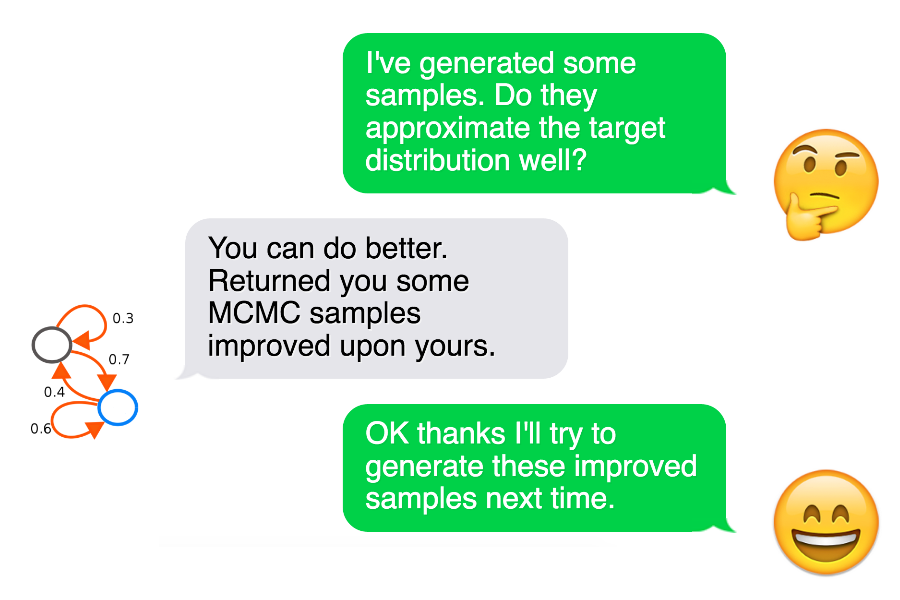
\includegraphics[width=0.6\linewidth]{Chapter5/amccartoon.png}
\caption{A cartoon illustration of the amortised MCMC idea in \cite{li:amcmc2017}. }
\label{fig:chap5_amc_cartoon}
\end{figure}

